\documentclass[11pt]{article}
\usepackage[margin=1in]{geometry}
\usepackage{amsmath,amssymb,amsthm}
\usepackage{graphicx}
\usepackage[hidelinks]{hyperref}

\newtheorem{theorem}{Theorem}
\newtheorem{definition}{Definition}
\newtheorem{remark}{Remark}

\newcommand{\BFPP}{\mathrm{BFPP}}

\title{Clopen ordinal towers and the ball fixed point property for \(C(K,p)\)}
\author{arXiv automatic math run \texttt{fa\_banach\_001}}
\date{2026-06-15}

\begin{document}
\maketitle

\section*{Source Question}

The source paper is Aviles--Japon--Lennard--Martinez-Cervantes--Stawski,
\emph{The ball fixed point property in spaces of continuous functions},
arXiv:2506.17995 \cite{source}.  It asks in final Question (i) whether there
is an infinite compact space \(K\) and a non-isolated point \(p\in K\) such
that
\[
  C(K,p)=\{f\in C(K):f(p)=0\}
\]
has the ball fixed point property \(\BFPP\).

\begin{center}
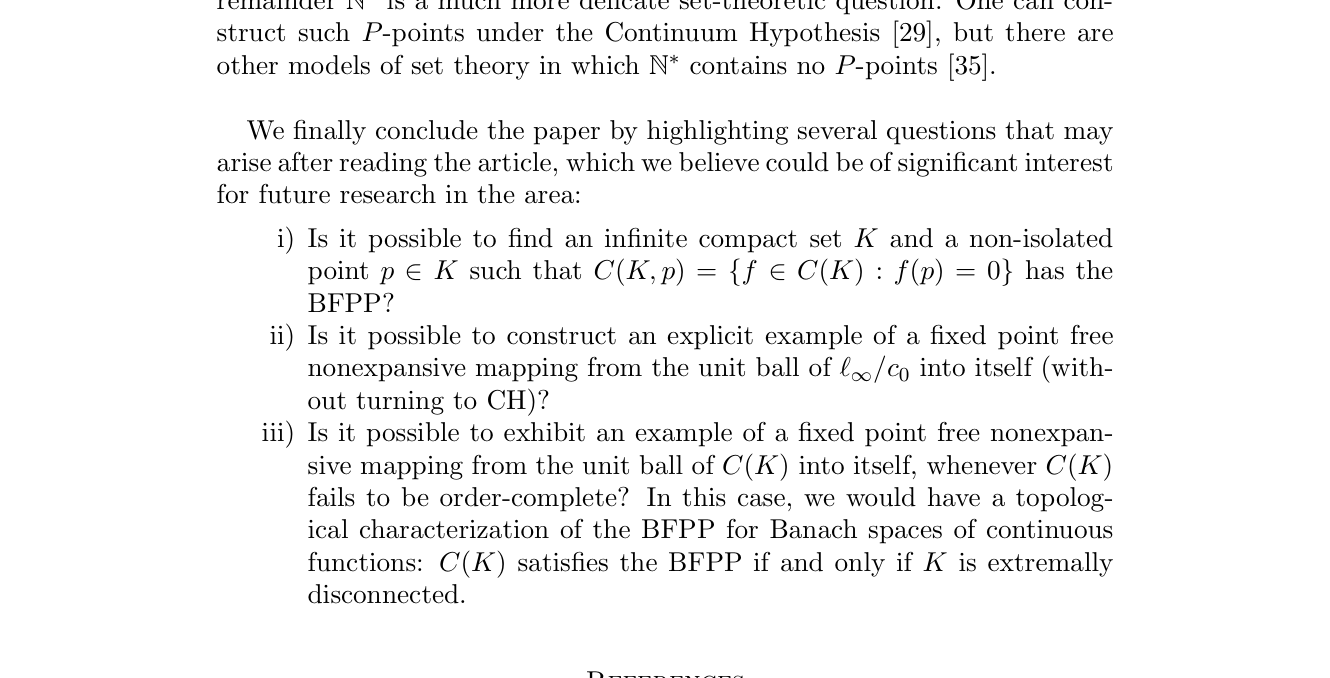
\includegraphics[width=\linewidth]{figures/open_question_i_crop.png}
\end{center}

The source paper proves failure when \(p\) is a non-\(P\)-point, and it also
constructs special \(P\)-point examples for which \(C(K,p)\) fails
\(\BFPP\).  A previous lane-15 packet proved failure for ordinal compacta
\([0,\kappa]\) at the endpoint.  The present packet records a reusable
well-ordered clopen-tower mechanism.

\section*{Definition}

\begin{definition}
Let \(K\) be compact Hausdorff and \(p\in K\).  A \emph{clopen ordinal tower}
at \(p\) is a family \((U_\alpha)_{\alpha<\kappa}\), where \(\kappa\) is a
nonzero limit ordinal, such that:
\begin{enumerate}
\item \(U_0=K\), and each \(U_\alpha\) is a clopen neighborhood of \(p\);
\item \(U_\beta\subset U_\alpha\) whenever \(\alpha<\beta<\kappa\);
\item \(U_\lambda=\bigcap_{\alpha<\lambda}U_\alpha\) for every nonzero limit
ordinal \(\lambda<\kappa\);
\item \(\bigcap_{\alpha<\kappa}U_\alpha=\{p\}\);
\item each annulus \(A_\alpha=U_\alpha\setminus U_{\alpha+1}\) is nonempty.
\end{enumerate}
\end{definition}

The continuity condition at limit stages implies that
\[
  K\setminus\{p\}=\bigsqcup_{\alpha<\kappa} A_\alpha.
\]
Indeed, if \(x\ne p\), the least \(\beta<\kappa\) such that
\(x\notin U_\beta\) cannot be \(0\) or a limit ordinal, hence
\(\beta=\alpha+1\) and \(x\in A_\alpha\).
Also, compactness implies that the tower is a neighborhood base at \(p\): if
\(V\) is an open neighborhood of \(p\), then the closed sets
\((K\setminus V)\cap U_\alpha\) cannot all be nonempty, since their total
intersection is empty.

\section*{Idea of the Proof}

Choose one point \(x_\alpha\in A_\alpha\) in each clopen annulus.  For
\(f\in C(K,p)\), define \(Tf\) to be constant on each annulus: put \(1\) on
the first annulus, shift the sampled value \(f(x_\alpha)\) to the next
annulus, and at a limit annulus put the ordinal limsup of the earlier sampled
values.  The annuli are clopen, so the only continuity issue is at \(p\).  But
if \(f(p)=0\), then \(f\) is small on a sufficiently deep tower neighborhood,
and all shifted and limsup values are small from that point onward.

The same formula is nonexpansive because point evaluations are contractive and
limsup is 1-Lipschitz with respect to the sup norm.  A fixed point would have
sampled value \(1\) on \(A_0\), then on every successor annulus by the shift,
and on every limit annulus by the limsup rule.  The sampled points converge to
\(p\), contradicting \(f(p)=0\).

\section*{Partial Result}

\begin{theorem}\label{thm:tower}
Let \(K\) be a compact Hausdorff space, let \(p\in K\), and suppose that \(p\)
admits a clopen ordinal tower.  Then \(C(K,p)\) fails the ball fixed point
property.
\end{theorem}

\begin{proof}
Let \((U_\alpha)_{\alpha<\kappa}\) be a clopen ordinal tower at \(p\), and
write \(A_\alpha=U_\alpha\setminus U_{\alpha+1}\).  Choose
\(x_\alpha\in A_\alpha\) for every \(\alpha<\kappa\).  We work over the real
scalar field, as in the source paper.

For a bounded scalar family \((a_\alpha)_{\alpha<\lambda}\) indexed by ordinals
below a nonzero limit \(\lambda\), write
\[
  \limsup_{\alpha\to\lambda} a_\alpha
  =
  \inf_{\gamma<\lambda}\sup_{\gamma<\alpha<\lambda} a_\alpha .
\]

Let \(X=C(K,p)\).  For \(f\in B_X\), define \(Tf\) by \((Tf)(p)=0\) and, for
\(x\in A_\beta\),
\[
  (Tf)(x)=c_\beta(f),
\]
where
\[
c_\beta(f)=
\begin{cases}
1, & \beta=0,\\
f(x_\alpha), & \beta=\alpha+1,\\
\displaystyle\limsup_{\alpha\to\beta} f(x_\alpha),
  & \beta<\kappa \text{ is a nonzero limit ordinal.}
\end{cases}
\]

First, \(Tf\) is continuous and belongs to \(B_X\).  It is constant on each
clopen annulus \(A_\beta\), and all constants lie in \([-1,1]\).  It remains
only to check continuity at \(p\).  Let \(\varepsilon>0\).  Since \(f(p)=0\)
and the tower is a neighborhood base at \(p\), there is \(\eta<\kappa\) such
that \(|f|<\varepsilon\) on \(U_\eta\).  If \(\beta>\eta\), then for successor
\(\beta=\alpha+1\) we have \(\alpha\ge\eta\), hence
\(|c_\beta(f)|=|f(x_\alpha)|<\varepsilon\).  If \(\beta>\eta\) is a limit
ordinal, the tail values \(f(x_\alpha)\), \(\eta<\alpha<\beta\), all have
absolute value \(<\varepsilon\), so
\(|c_\beta(f)|\le\varepsilon\).  Hence \(|Tf|<\varepsilon\) on a sufficiently
deep \(U_\delta\), and \(Tf\) is continuous at \(p\).

The map \(T:B_X\to B_X\) is nonexpansive.  Let \(f,g\in B_X\) and set
\(d=\|f-g\|_\infty\).  On \(A_0\), \(Tf-Tg=0\).  On a successor annulus
\(A_{\alpha+1}\),
\[
  |c_{\alpha+1}(f)-c_{\alpha+1}(g)|
  =
  |f(x_\alpha)-g(x_\alpha)|
  \le d.
\]
For a nonzero limit \(\lambda<\kappa\), the elementary inequality
\[
 \left|
 \limsup_{\alpha\to\lambda} f(x_\alpha)
 -
 \limsup_{\alpha\to\lambda} g(x_\alpha)
 \right|
 \le
 \sup_{\alpha<\lambda}|f(x_\alpha)-g(x_\alpha)|
\]
gives \(|c_\lambda(f)-c_\lambda(g)|\le d\).  Therefore
\(\|Tf-Tg\|_\infty\le d\).

Finally suppose that \(f\in B_X\) is a fixed point of \(T\).  Since \(Tf\) is
constant on \(A_\alpha\), we have \(f(x_\alpha)=c_\alpha(f)\).  Transfinite
induction gives \(f(x_\alpha)=1\) for every \(\alpha<\kappa\).  The initial
step is \(f(x_0)=c_0(f)=1\).  If \(f(x_\alpha)=1\), then
\[
  f(x_{\alpha+1})=c_{\alpha+1}(f)=f(x_\alpha)=1.
\]
If \(\lambda<\kappa\) is a nonzero limit ordinal and the conclusion holds for
all \(\alpha<\lambda\), then
\[
  f(x_\lambda)=c_\lambda(f)
  =
  \limsup_{\alpha\to\lambda} f(x_\alpha)
  =
  1.
\]
But the net \((x_\alpha)_{\alpha<\kappa}\) converges to \(p\), because for
every \(\eta<\kappa\) and every \(\alpha\ge\eta\), \(x_\alpha\in U_\eta\).
Continuity of \(f\) at \(p\) therefore forces
\[
  1=\lim_{\alpha\to\kappa} f(x_\alpha)=f(p)=0,
\]
a contradiction.  Thus \(T\) has no fixed point, and \(C(K,p)\) fails
\(\BFPP\).
\end{proof}

\section*{Scope and Limitations}

Theorem~\ref{thm:tower} is a genuine \(P\)-point-side obstruction whenever a
well-ordered clopen tower exists.  It does not settle the source question in
full, because a non-isolated \(P\)-point need not come equipped with such a
tower or with a norm-one retract onto a tower model.  The arbitrary
non-isolated \(P\)-point case remains the hard core of the problem.

\section*{Novelty and Verification Notes}

The local run indexes were searched for arXiv \texttt{2506.17995}, BFPP,
\(C(K,p)\), \(P\)-points, and clopen tower language.  The only relevant prior
run materials were the lane-15 ordinal compact partial packet and the
unfinished full-push attempt.  This packet promotes the clopen-tower route from
that attempt into a precise partial theorem.

Human review should focus on two points: the continuity of \(Tf\) at \(p\),
and the 1-Lipschitz estimate for the limsup operation at limit annuli.

\begin{thebibliography}{9}
\bibitem{source}
A. Aviles, M. Japon, C. Lennard, G. Martinez-Cervantes, A. Stawski,
\emph{The ball fixed point property in spaces of continuous functions},
arXiv:2506.17995, 2025.
\end{thebibliography}

\end{document}
